\chapter{Brute Force Dispositivi mobile}
In questo capitolo andremo a discutere di come viene eseguito un Brute-Force sui dispositivi mobile.

\section{Brute Force con Dispositivi mobile}

Una delle metodologie possibili da applicare per eseguire un Brute-Force sui dispositivi mobile è quella di utilizzare un'altro device mobile per eseguire l'attacco, questo è possibile grazie all'installazione di NetHunter sul device attaccante, un sistema operativo che ci permetterà di abilitare determinate operazioni eseguibili sul dispositvo.

\subsection{NetHunter}

NetHunter\cite{NetHunter} è una ROM per Android sviluppata appositamente per chi vuole utilizzare i programmi presenti nella distribuzione Kali Linux da telefono.

NetHunter permette quindi di interfacciarsi con i vari strumenti per testare la sicurezza informatica. Nei software a disposizione si troveranno diversi programmi per effettuare attacchi di tipo HID Keyboard, BadUSB, Evil AP MANA e molto altro. 

Kali NetHunter è disponibile per dispositivi senza root (NetHunter Rootless), per dispositivi rooted (NetHunter Lite / NetHunter).

\begin{figure}[h!]
    \centering
    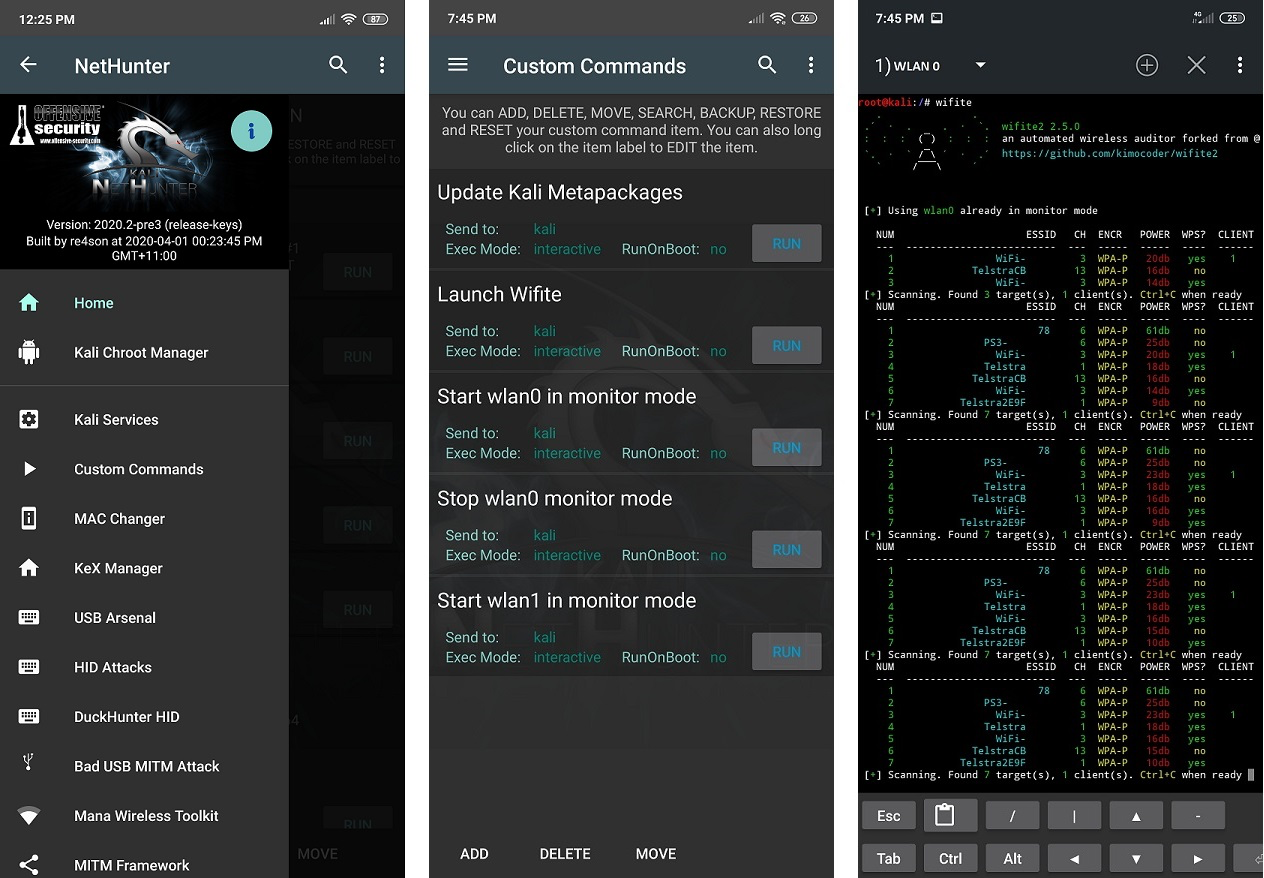
\includegraphics[width=116mm]{Immagini/3/nethunter_1.png}
    \caption{NetHunter}
    \label{fig:NetHunter}
\end{figure}

\newpage

Nel nostro caso andremo ad utilizzare la versione NetHunter, che ci permetterà di utilizzare l'interfaccia HID\footnote[1]{\textbf{HID} : Human Interface Device o HID è un tipo di dispositivo informatico solitamente utilizzato dagli esseri umani che riceve input dagli umani e fornisce output agli umani.}, questa permetterà al dispositivo attaccante di comunicare con il dispositivo vittima, come se fosse un mouse o una tastiera.

\subsection{Android-PIN-Bruteforce}

La prima tecnica che andremo a vedere è Android-PIN-Bruteforce\cite{Android-PIN-Bruteforce} che è stato sviluppato dal gruppo urbanadventur, qui si andrà a frutture l’interfaccia HID per simulare l’utilizzo di una tastiera per l’inserimento dei PIN, permettendo di provare tutti i PIN possibili in circa 16 ore.

Per eseguire questo tipo di attacco dobbiamo essere in possesso di un dispositivo mobile che sia compatibile per via ufficiali\cite{nethunter_official} o mantenuto dalla community\cite{nethunter_community}. Una volta che si ha il dispositivo bisogna installarci Nethunter su di esso in modo da abilitare l'interfaccia HID.

L'ultima due cose necessarie per eseguire l'attacco sono un cavo OTG (maschio micro USB  -> femmina USB-A) e il dispositivo vittima con il suo cavo di ricarica.

\begin{figure}[h!]
    \centering
    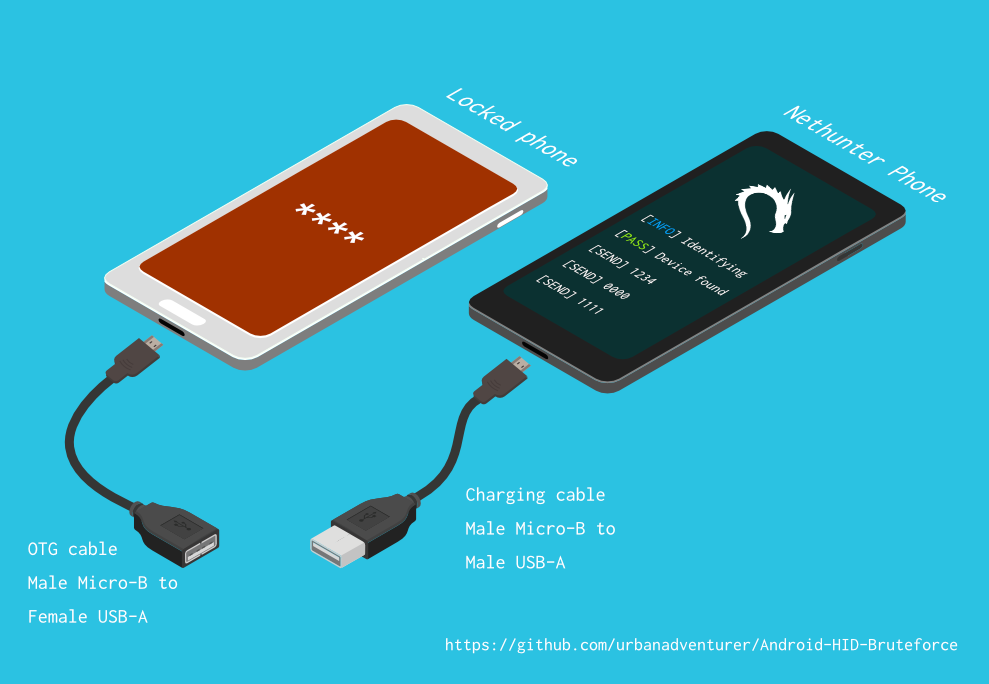
\includegraphics[width=140mm]{Immagini/3/pin_brute_1.png}
    \caption{Android-PIN-Bruteforce}
    \label{fig:Android-PIN-Bruteforce}
\end{figure}

Questa tecnica permette di :
\begin{itemize}
	\item A differenza di altri metodi, non è necessario abilitare il debug ADB o USB sul telefono bloccato, inoltre si può impostare la lunghezza della password da provare (da 1 a 10).
	\item Il telefono Android bloccato non ha bisogno di essere rootato
	\item Trasforma il tuo telefono NetHunter in una macchina per crackare il PIN Android
	\item Non è necessario acquistare hardware speciale
	\item Utilizza i file di configurazione per supportare diversi telefoni
	\item Elenchi di PIN ottimizzati per PIN a 3,4,5 e 6 cifre
	\item Ignora i popup del telefono incluso l’avviso di basso consumo
	\item Rileva quando il telefono è scollegato o spento e attende mentre riprova ogni 5 secondi
	\item Ritardi configurabili di N secondi dopo ogni X tentativi di PIN
\end{itemize}

Per eseguire il seguente script, basta scaricarlo dal git ufficiale del gruppo e collegare il dispositivo attacante al dispositivo vittima come detto in precedenza e lanciare dal terminale del dispositivo il comando :

\begin{lstlisting}[ caption={Android-PIN-Bruteforce command}, style=javaScriptCode]
	bash ./android-pin-bruteforce crack
\end{lstlisting}

\begin{figure}[h!]
    \centering
    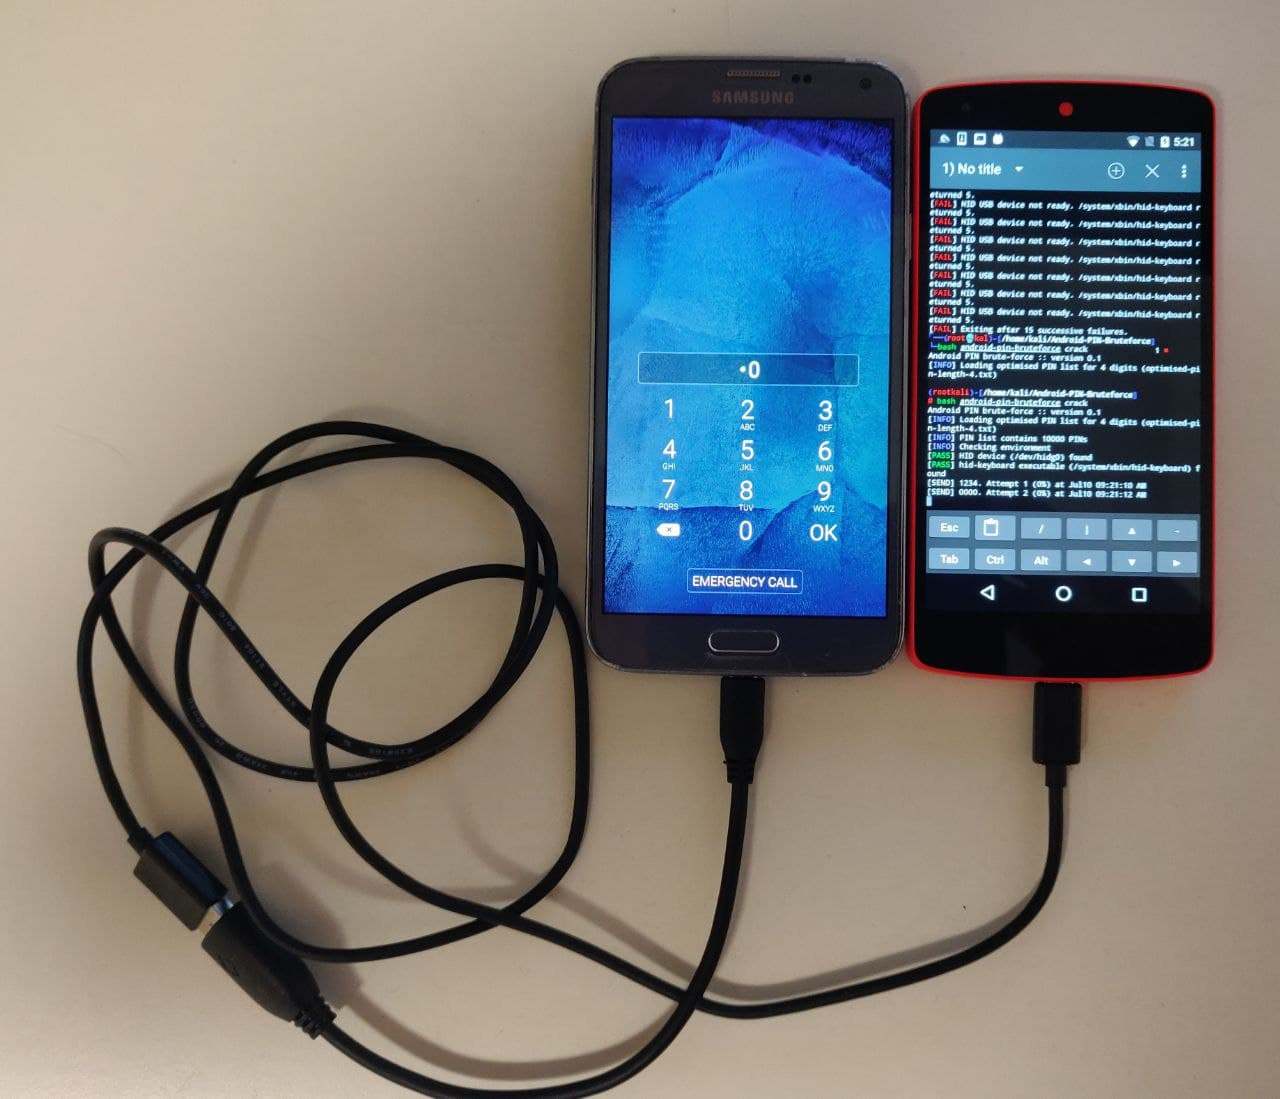
\includegraphics[width=140mm]{Immagini/3/brute.jpg}
    \caption{Android-PIN-Bruteforce}
    \label{fig:Android-PIN-Bruteforce}
\end{figure}

Questo script come detto, fa uso di una serie di liste di PIN ottimizzate (Gli elenchi di PIN ottimizzati sono stati generati estraendo le password numeriche dalle perdite di database e quindi ordinandole in base alla frequenza). Per la scelta della lunghezza dei PIN da utilizzare, basta aggiungere il comando –lenght X, dove X sta per la lunghezza della password da utilizzare.

Inoltre è possibile utilizzare delle maschere per i PIN da utilizzare :
\begin{itemize}
	\item Per provare tutti gli anni dal 1900 al 1999 \newline
	\begin{lstlisting}[ caption={Android-PIN-Bruteforce command musk}, style=javaScriptCode]
		bash ./android-pin-bruteforce crack -mask "19.."
	\end{lstlisting}
	\item Per provare i PIN che hanno un 1 nella prima cifra e un 1 nell’ultima cifra \newline
	\begin{lstlisting}[ caption={Android-PIN-Bruteforce command musk}, style=javaScriptCode]
		bash ./android-pin-bruteforce crack -mask "1..1"
	\end{lstlisting}
	\item Per provare i PIN che terminano con 4 o 5, usa \newline
	\begin{lstlisting}[ caption={Android-PIN-Bruteforce command musk}, style=javaScriptCode]
		bash ./android-pin-bruteforce crack -mask ...[45]
	\end{lstlisting}
\end{itemize}

I produttori di dispositivi creano le proprie schermate di blocco diverse da quelle predefinite o di serie di Android, per specificare una predefinita configurazione, bisogna aggiungere il comando –config ConfingFile, che permette di adattare i comandi inviati in base alla configurazione del dispositivo vittima.

Una funzione importante è il fatto che il dispositivo attacante in automatico ogni X tentativi si metterà in pausa, simulando il time out dovuto ai vari tentativi falliti.

\begin{figure}[h!]
    \centering
    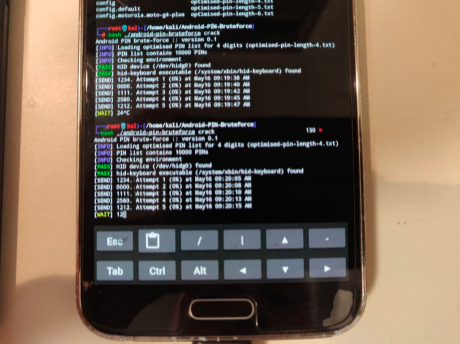
\includegraphics[width=100mm]{Immagini/3/time_out.png}
    \caption{Android-PIN-Bruteforce time out}
    \label{fig:Android-PIN-Bruteforce}
\end{figure}

Una delle problematiche di questo script è il fatto che non sia in grado di riconsocere quando il PIN che abbiamo utilizzato avrà successo, infatti lui, anche dopo aver sbloccato il dispositivo continuerà con i vari tentativi.

\section{WBRUTE}

Un’altra tecnica testata è quella WBRUTE\cite{wbrute}, sviluppata da wuseman. Questa è molto diversa e molto più potente da quella vista in precedenza, per diversi fattori :

\begin{itemize}
	\item Funzionante solo se il dispositivo vittima ha una versione Android 8.0
	\item Permette di bypassare il time out dopo X tentativi errati
	\item Deve essere abilitato ADB nel dispositivo vittima
	\item Deve essere dato l’accesso al dispositivo attaccante dal dispositivo vittima
	\item Permette di sapere il PIN corretto
	\item Permette di sostituire il PIN con uno nuovo
	\item Utilizzabile con PIN di 4 o 6 cifre
	\item Il dispositivo vittima deve essere rootato
\end{itemize}

Questa tecnica sfrutta una vulnerabilità introdotto con Android 8.0, nata dalla rimozione della possibilità di impostare come PIN l’orario attuale, per un errore è stato lasciato il comando locksettings che permette di eseguire operazioni sul PIN, in questo caso di proverà a rimuovere il PIN corretto, andando a catturare il messaggio di successo in modo da avere una conferma che il PIN sia corretto.

Il comando eseguito è :

\begin{lstlisting}[ caption={Android-PIN-Bruteforce command}, style=javaScriptCode]
	adb shell locksettings clear -old $i | grep "Lock credential cleared"
\end{lstlisting}

Dove \$i è il valore che verrà testato (da 0000 a 9999). Una volta trovato il PIN questo ci verrà mostrato a schermo sul device attacante e richiesto se si vuole modificare con un’altro. Questa tecnica permette di provare tutti e 9999 PIN in poco più di un’ora grazie al fatto che non si ha il problema del time out, ma come detto in precedenza, questa tecnica è poco applicabilile, per il fatto che si deve avere un dispositivo bloccato con Android 8.0, debug USB attivo e autorizzazione per il device attacante.

Il tutto è Funzionante grazie allo strumento adb\cite{adb} che permette l’esecuzione di comandi direttamente sul dispositivo.


\section{CiLocks}

\section{Arkhota}



